% !TEX root = ../main.tex
\chapter{算法在移动平台的实现}
本文方法用OpenGL Compute Shader实现,所以理论上可以在任何支持OpenGL 4.3及以上版本的设备上运行。为了验证这一点,我们将本文方法应用到了哇陶中。哇陶是一款安卓平台上的陶瓷制作模拟软件。用户可以借助该软件体验陶瓷制作全过程\footnote{不同的瓷器,制作步骤会有所区别。哇陶中的过程与常用的青花瓷制作过程保持一致,即泥胚塑形、烧制、贴花、落款、烤花。},软件截图如\autoref{fig:watao}所示。如果用户对自己制作的瓷器感到很满意,还可以通过\autoref{subfig:watao_5}所示界面下单购买。

\begin{figure}[htbp]
	\centering
	\begin{subfigure}[b]{.32\textwidth}
		\centering
		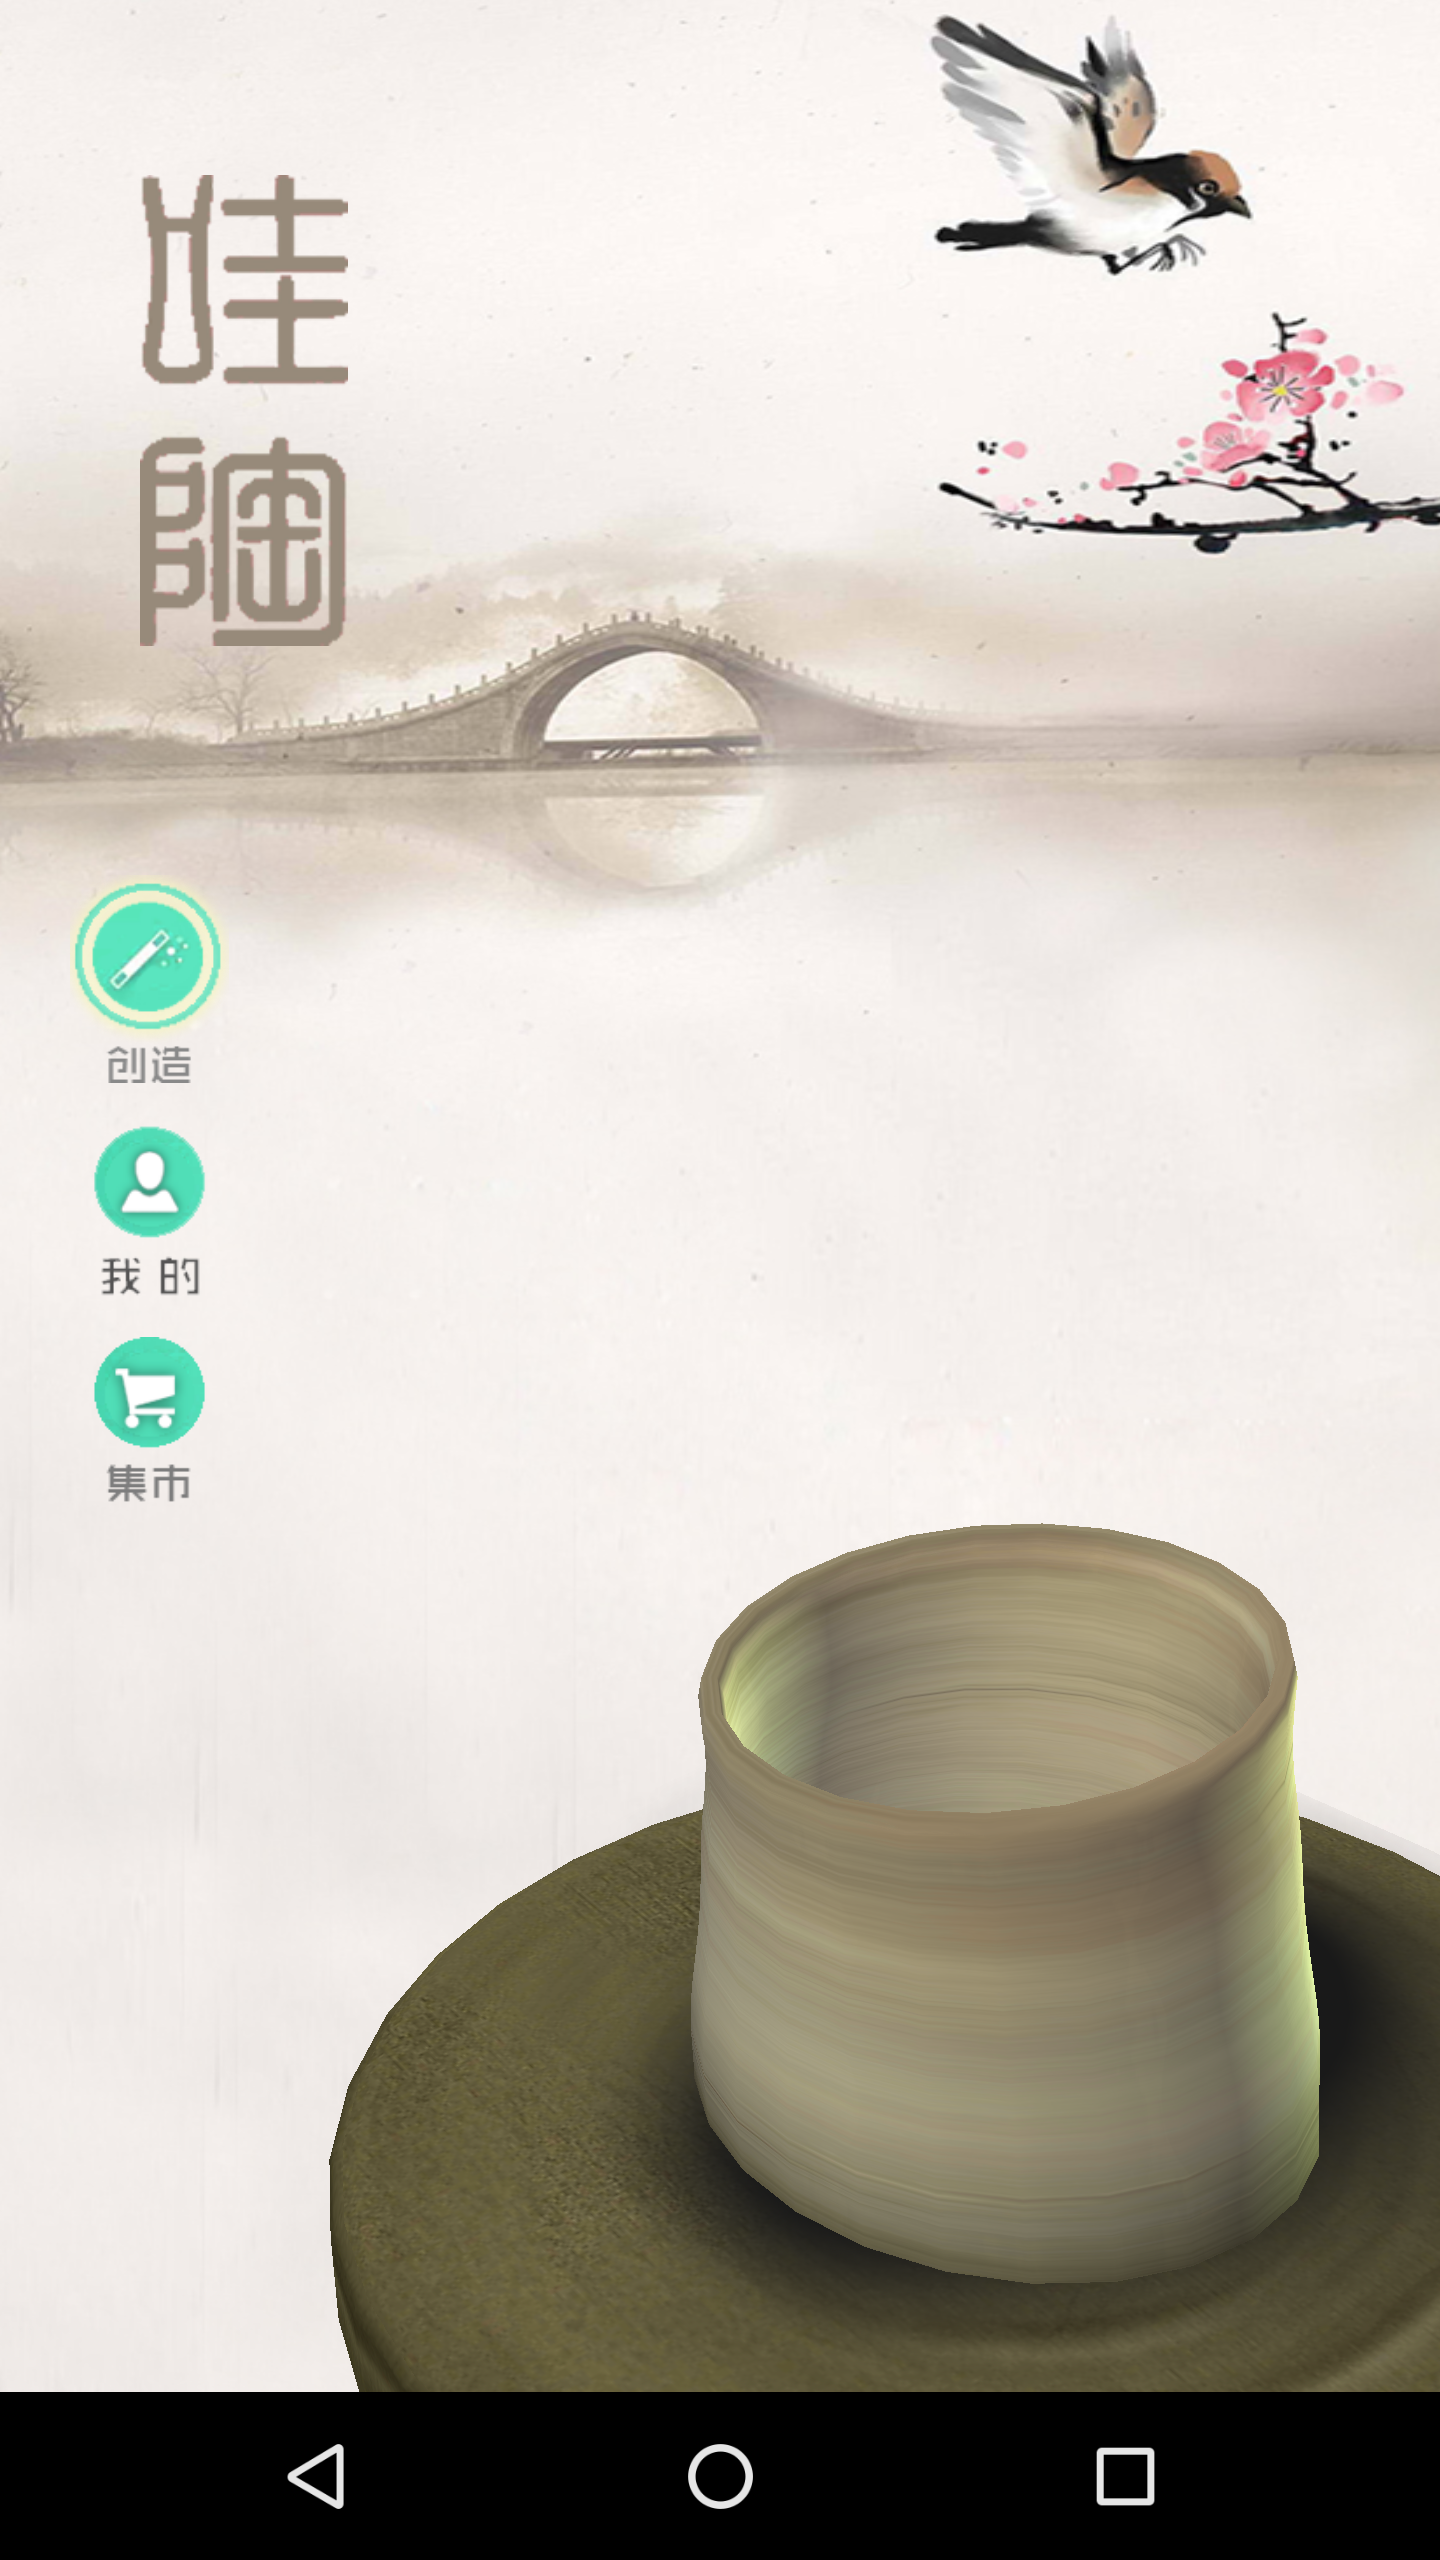
\includegraphics[width = \textwidth]{watao_0.png}
		\caption{初始界面}\label{subfig:watao_0}
	\end{subfigure}
	\begin{subfigure}[b]{.32\textwidth}
		\centering
		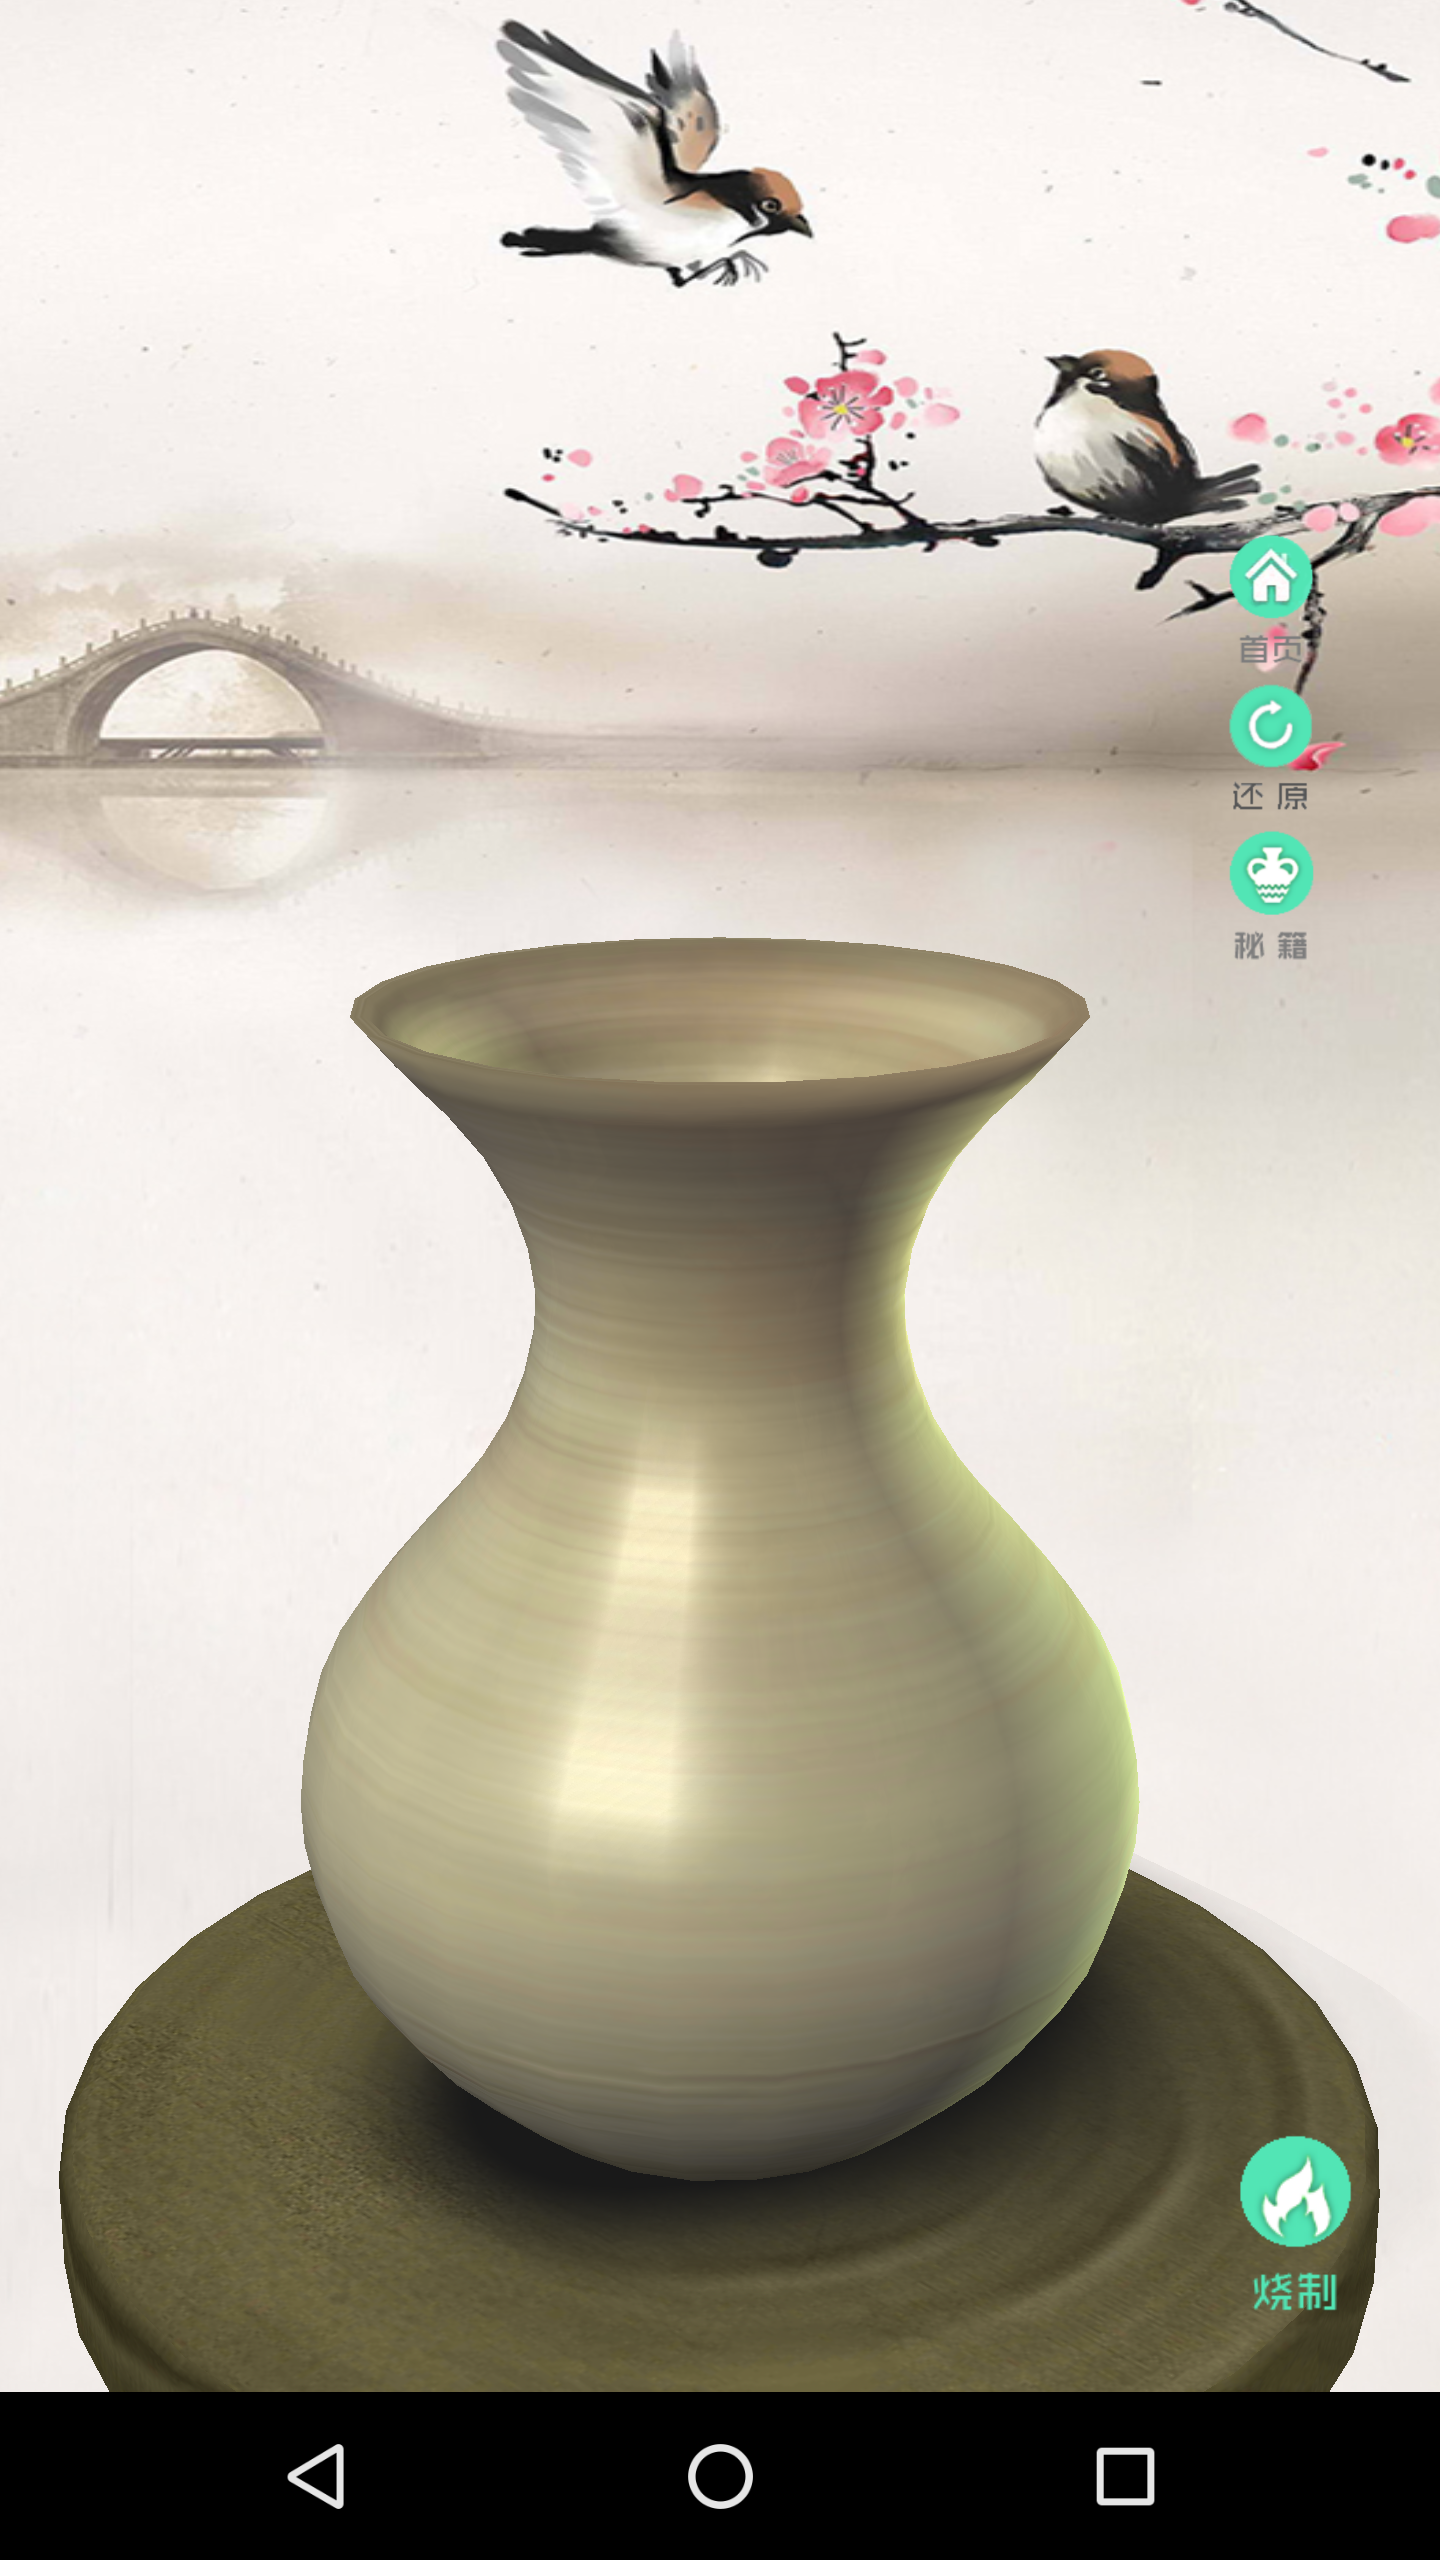
\includegraphics[width = \textwidth]{watao_1.png}
		\caption{拉胚界面}\label{subfig:watao_1}
	\end{subfigure}
	\begin{subfigure}[b]{.32\textwidth}
		\centering
		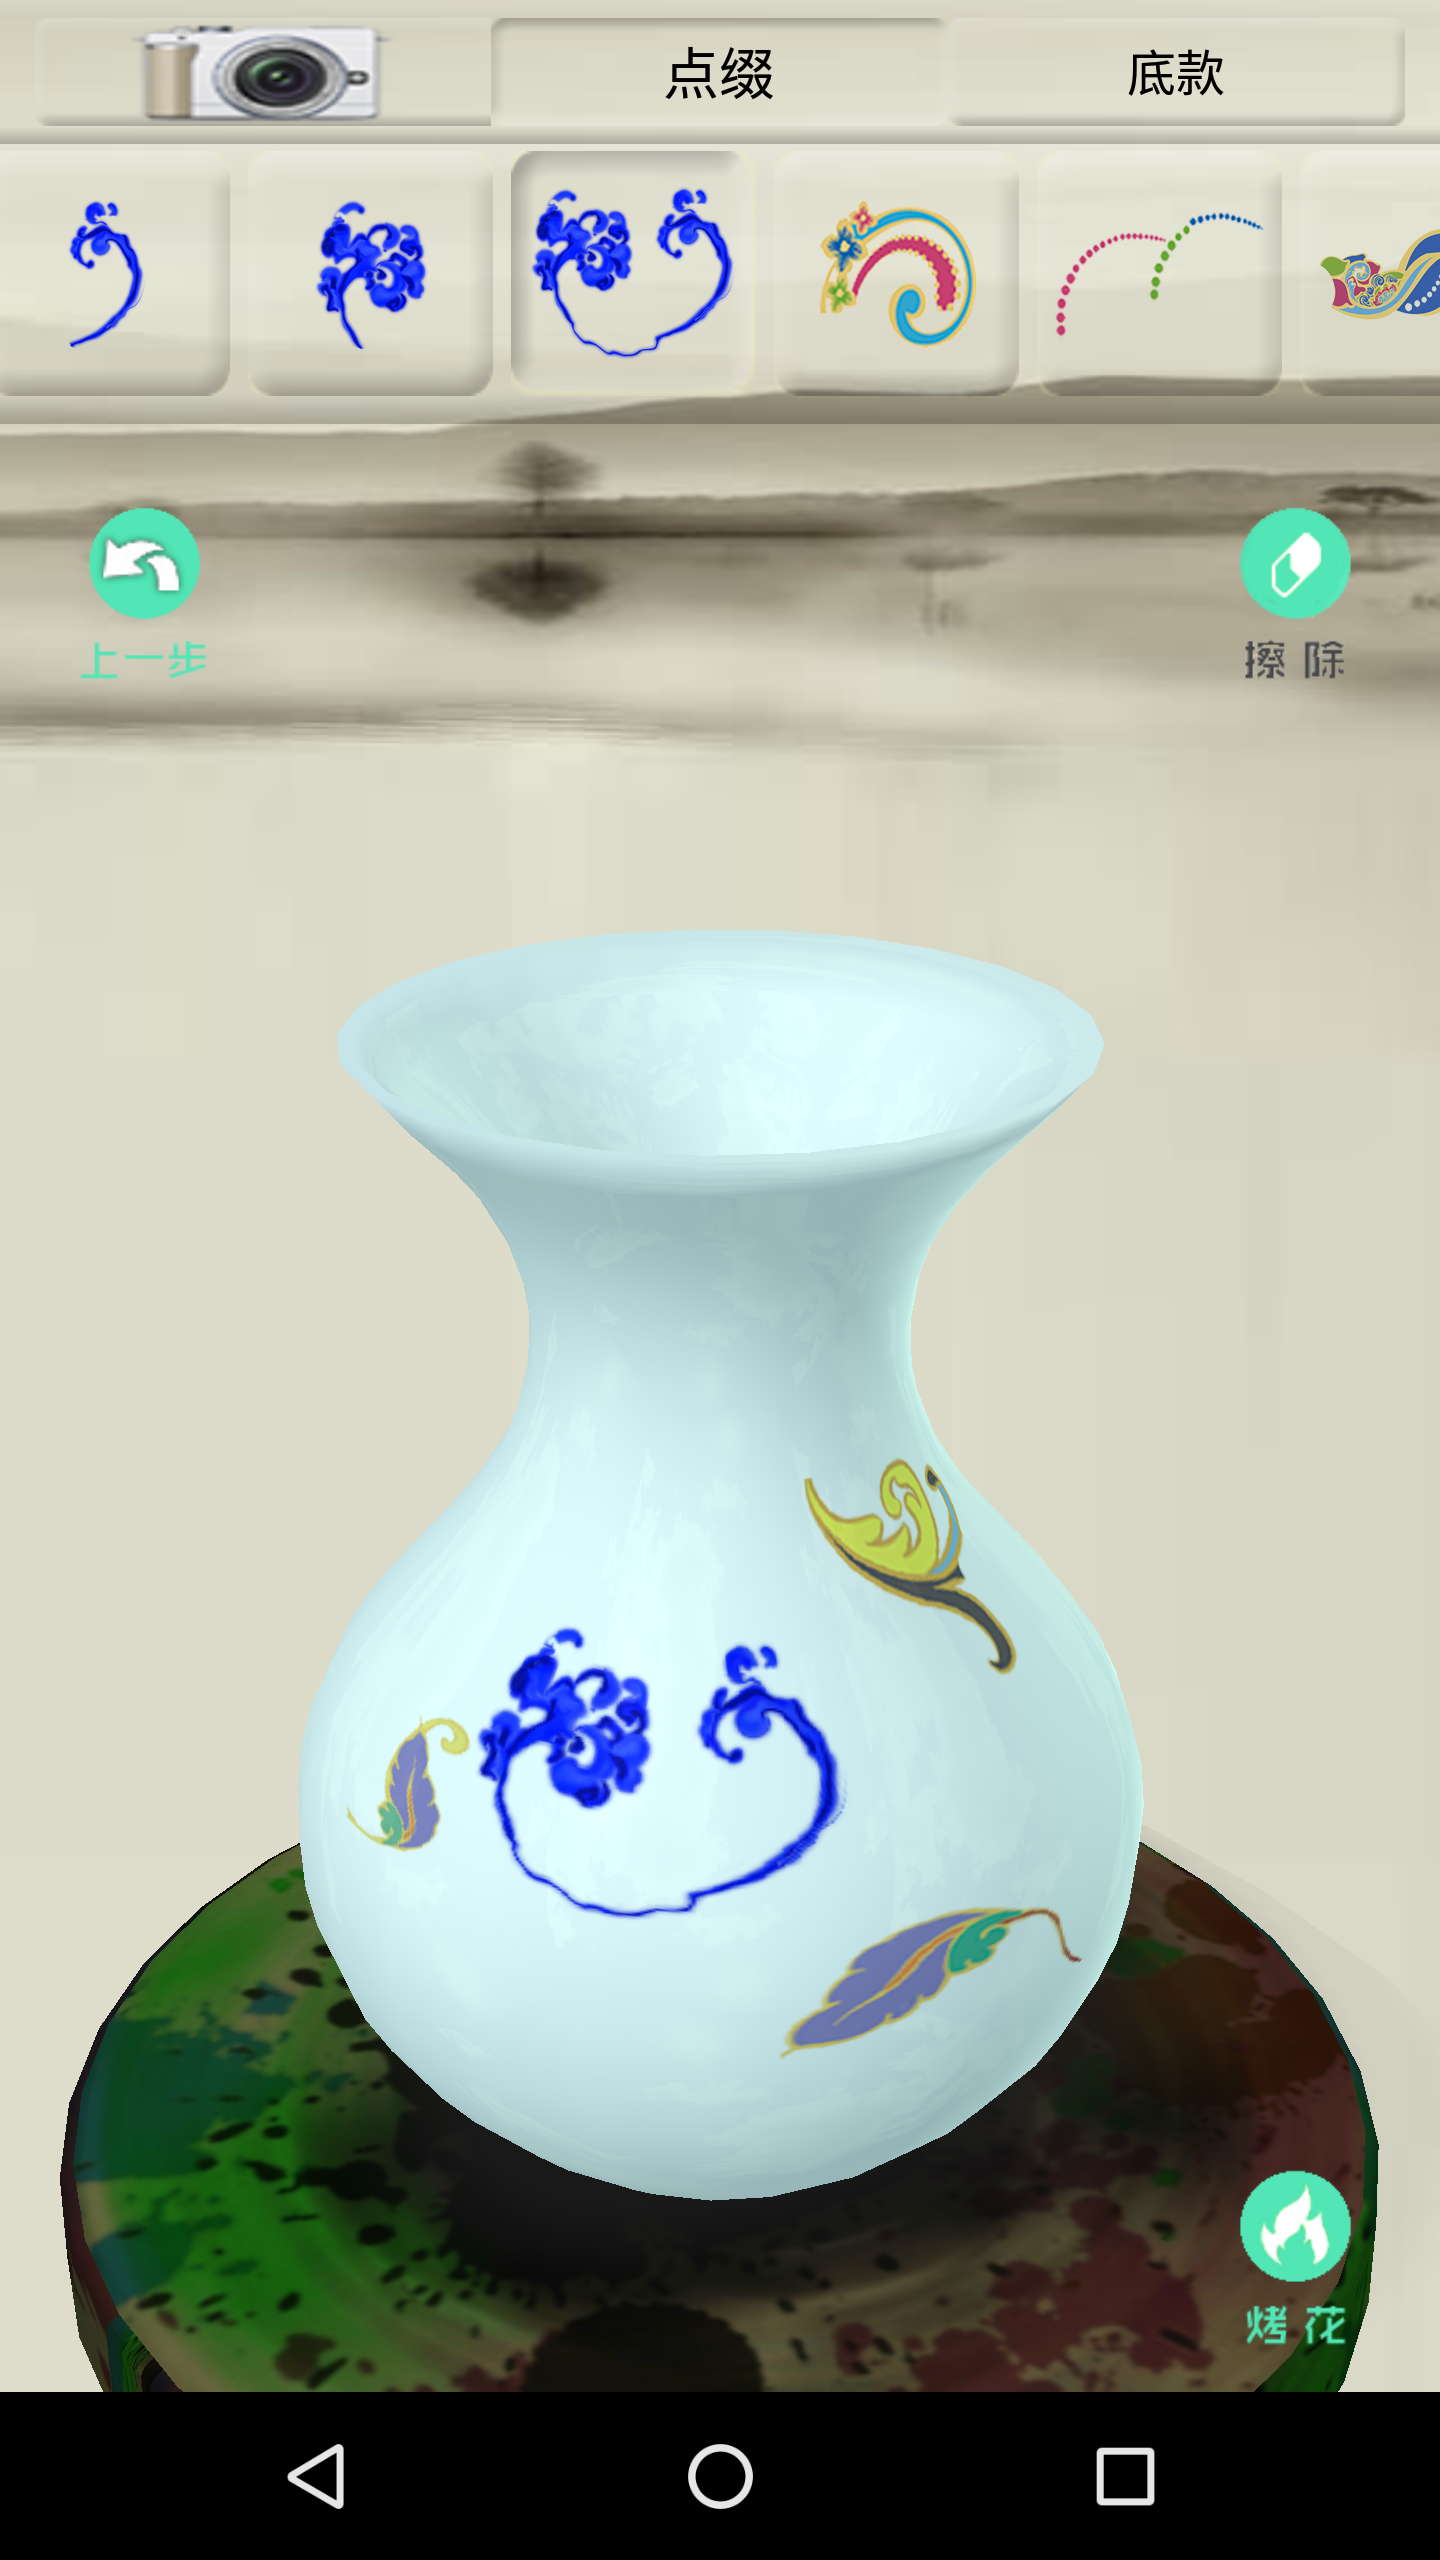
\includegraphics[width = \textwidth]{watao_2.png}
		\caption{贴图界面}\label{subfig:watao_2}
	\end{subfigure}

    \par
	\begin{subfigure}[b]{.32\textwidth}
		\centering
		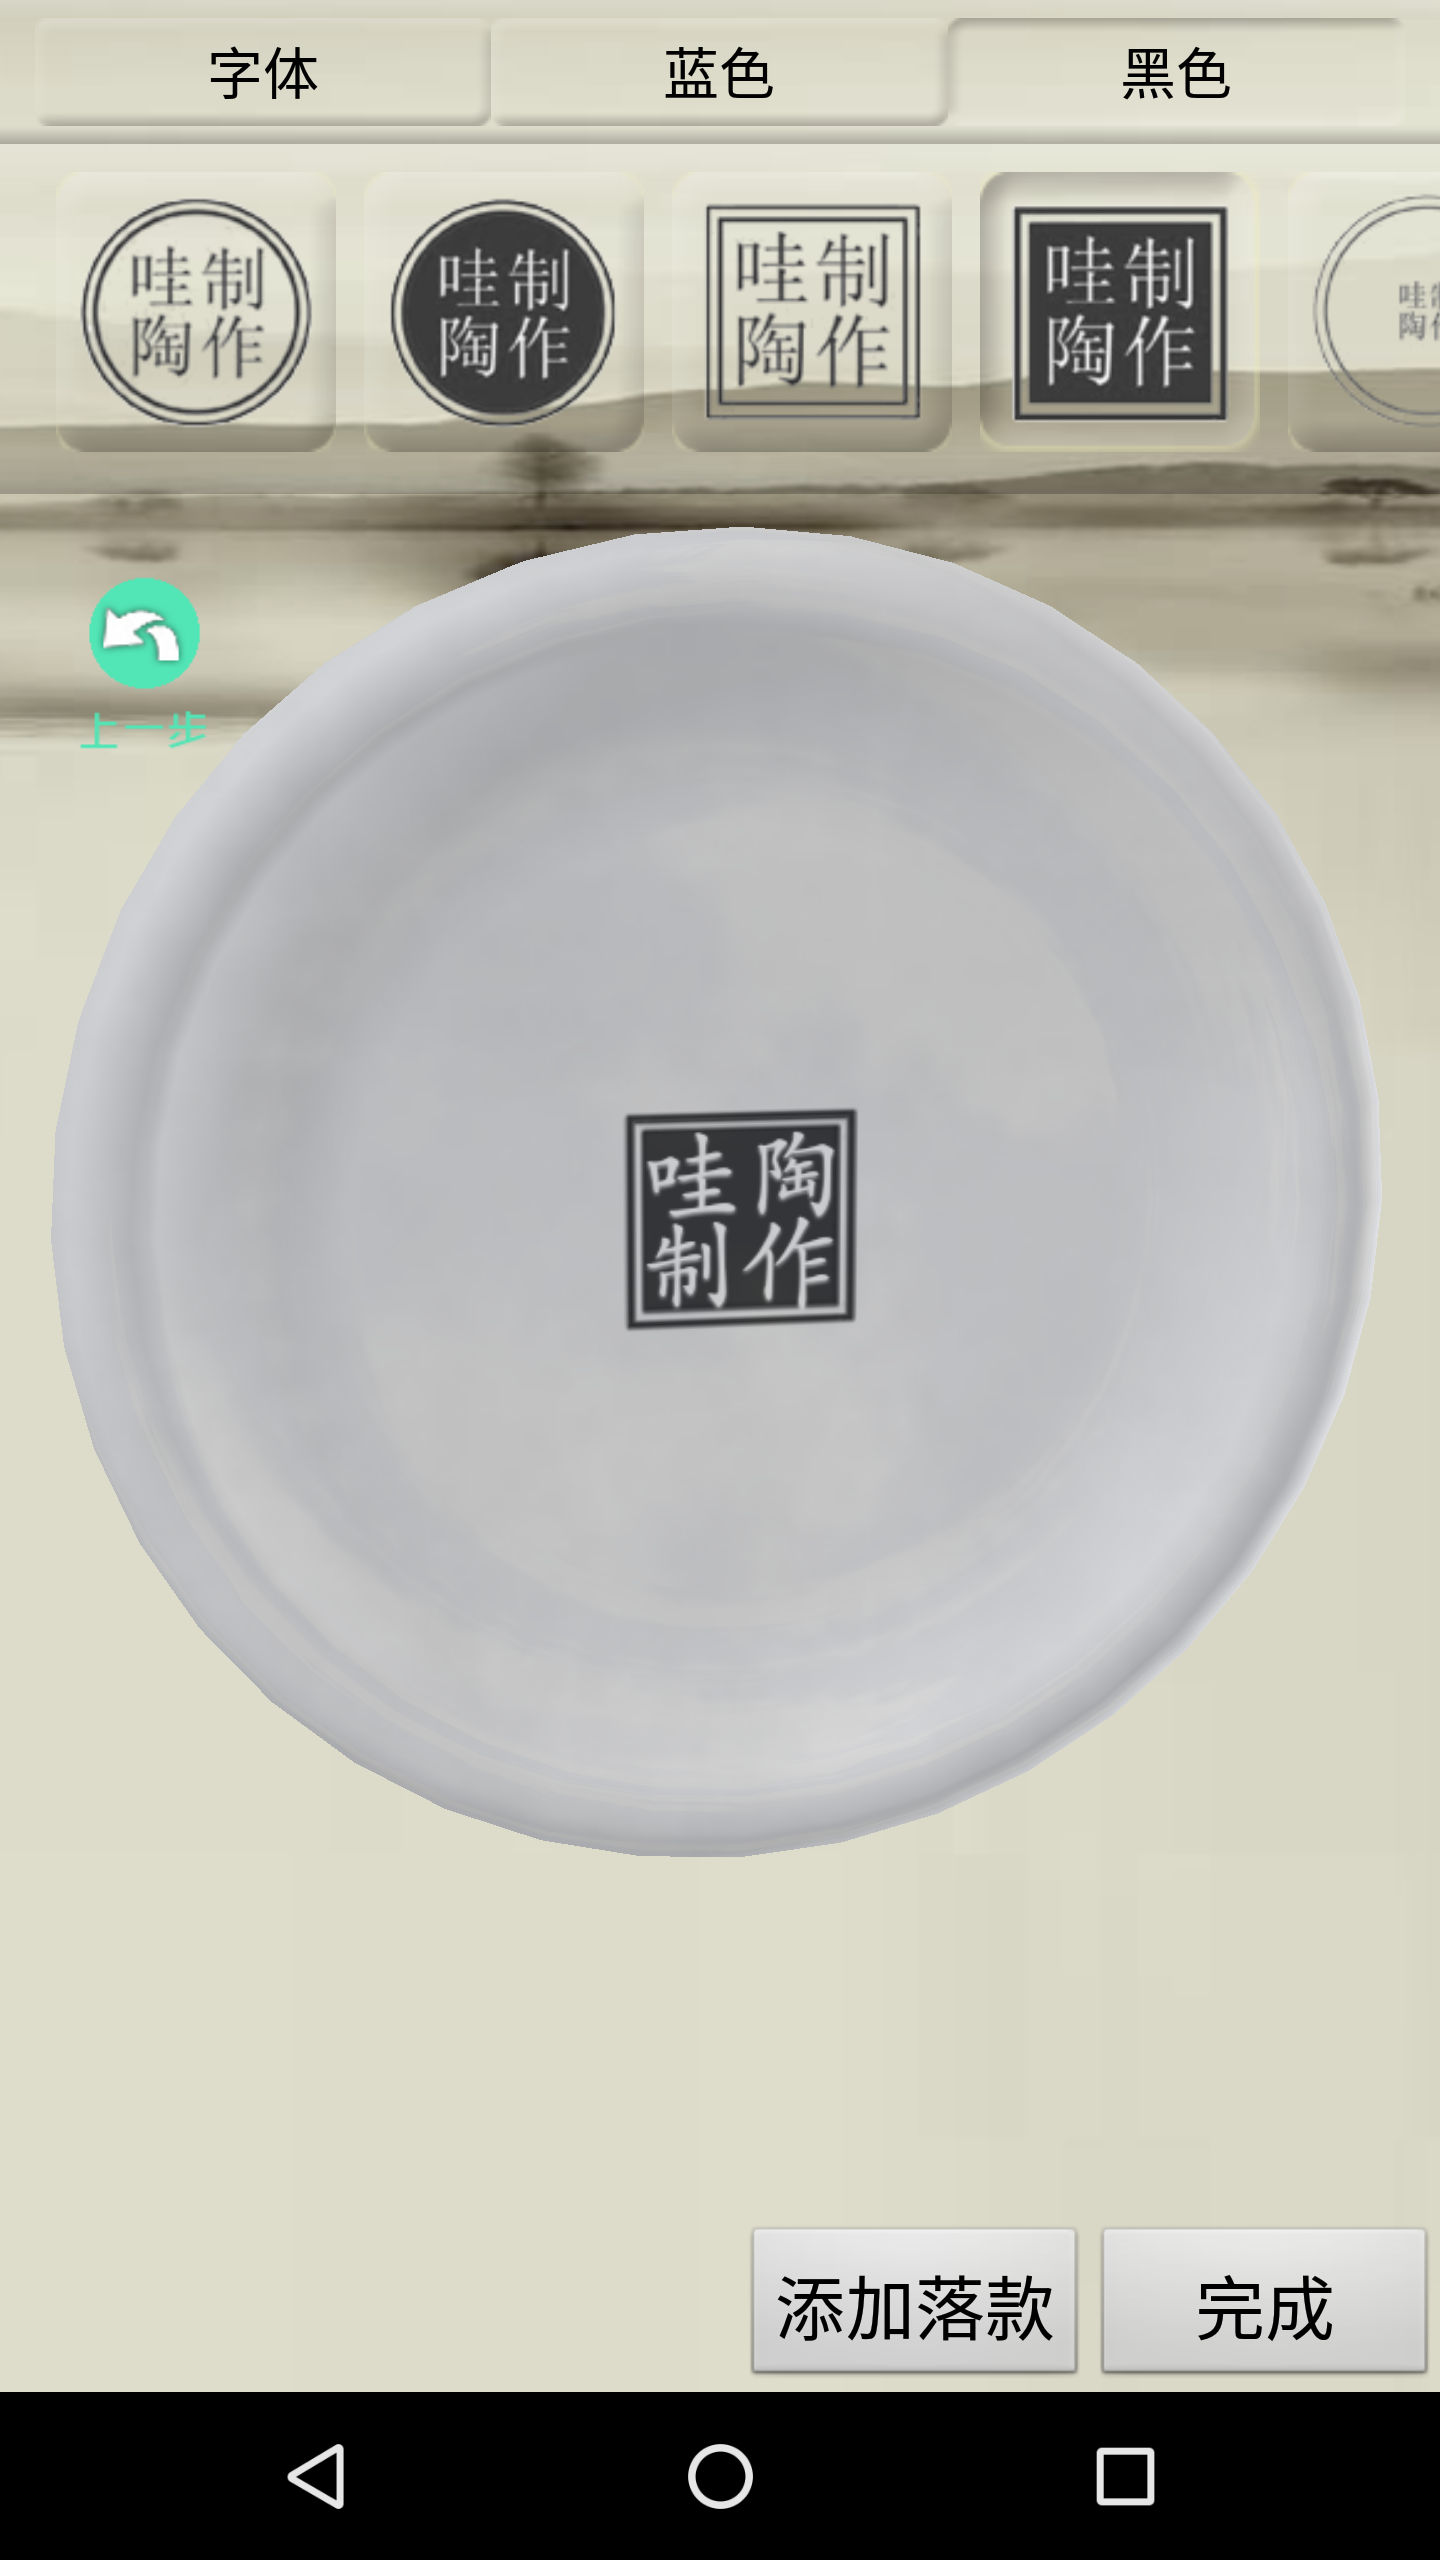
\includegraphics[width = \textwidth]{watao_3.png}
		\caption{落款界面}\label{subfig:watao_3}
	\end{subfigure}
	\begin{subfigure}[b]{.32\textwidth}
		\centering
		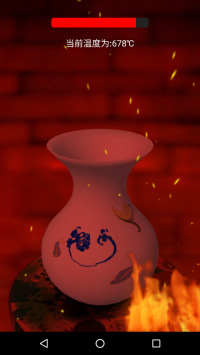
\includegraphics[width = \textwidth]{watao_4.png}
		\caption{烤花界面}\label{subfig:watao_4}
	\end{subfigure}
	\begin{subfigure}[b]{.32\textwidth}
		\centering
		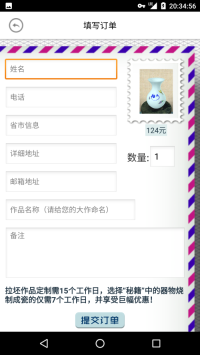
\includegraphics[width = \textwidth]{watao_5.png}
		\caption{购买界面}\label{subfig:watao_5}
	\end{subfigure}

	\caption{哇陶截图}\label{fig:watao}
\end{figure}

在真实的陶瓷制作过程中,泥胚塑形阶段制作陶瓷的工匠不仅可以通过转台将瓷器拉成一个完全对称的旋转体,如\autoref{sub:pottery_shape_0}所示,还可以通过手工捏胚将瓷器塑造成更具创造性的形状,如\autoref{sub:pottery_shape_0}所示。其中拉胚过程在软件中较容易模拟,略过不述。手工捏胚过程通过本文方法实现,以帮助用户得到满意的造型。

\begin{figure}[htbp]
	\centering
	\begin{subfigure}[b]{.4\textwidth}
		\centering
		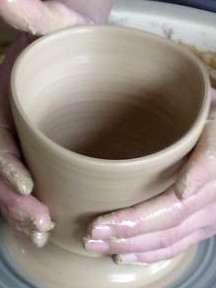
\includegraphics[width = \textwidth]{pottery_shape_0.jpg}
		\caption{转盘拉胚}\label{subfig:pottery_shape_0}
	\end{subfigure}
	\begin{subfigure}[b]{.4\textwidth}
		\centering
		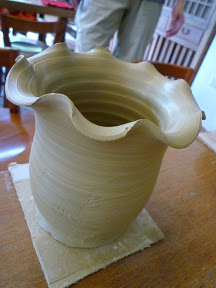
\includegraphics[width = \textwidth]{pottery_shape_1.jpg}
		\caption{莲花口}\label{subfig:pottery_shape_1}
	\end{subfigure}
	\caption{泥胚塑形}\label{fig:pottery_shape}
\end{figure}

由于安桌手机没有鼠标键盘,其主要交互手段为触控,且手机屏幕相对于桌面显示器要小很多。所以本文方法的交互方式\footnote{本文方法需要先选定控制顶点,然后通过位移控制顶点来变形模型。}并不适合手机用户,尤其是的选定控制顶点的阶段,用户因为手机屏幕小,手指点击精度低,而以体为变形空间控制顶点数目以多,所以用户很难快速准确的选点。

为了解决这一问题,本文采用了直接自由变形\cite{hsu1992}以改善交互。直接自由变形允许用户指定模型中某些点变形后的空间位置,然后以这些点变形前后的位移为约束,以最小化控制顶点的位移为优化条件,用约束优化方法反求出所有控制顶点的位移。再以新的控制顶点变形整个模型。在该方法中,用户输入的位移与模型的变形在着较为明确的对应关系,使得自由变形算法更为简单易用。最为关键的是该方法无需在变形之前选择控制顶点,正好弥补了前方所述的本文方法在手机中选点所产生的交互问题。

并且我们观察到,用户比较倾向于捏制一些对称的器型。所以我们还在直接变形的基础了提供了“对称变形”的功能。如用户选择模型上的点$P$变形前后的位移是$V$,$P$的空间位置是$(P_x, P_y, P_z)$,微量V为$(V_x, V_y, V_z)$。那么我们可以将$P$,$V$关于$Y$\footnote{$Y$轴即为瓷器从底部到顶部的方向}轴做一个中心对称。得到$V'$和$P'$分别为$(-P_x, P_y, -P_z)$,$(-V_x, V_y, -V_z)$。这样我们就可以以$P$,$P'$的位置和位移为输入进行直接自由变形,以等到对称的变形结果。用户还可以选择多生成几个对称的点,以生成更加繁复的对称图案。
